\preClass{Coordinate Systems}


\videoLink{Section 4.5 day 2}{https://www.youtube.com/playlist?list=PLYHZK3b8UFw0U_iMosD8HZraus76s5k2i}

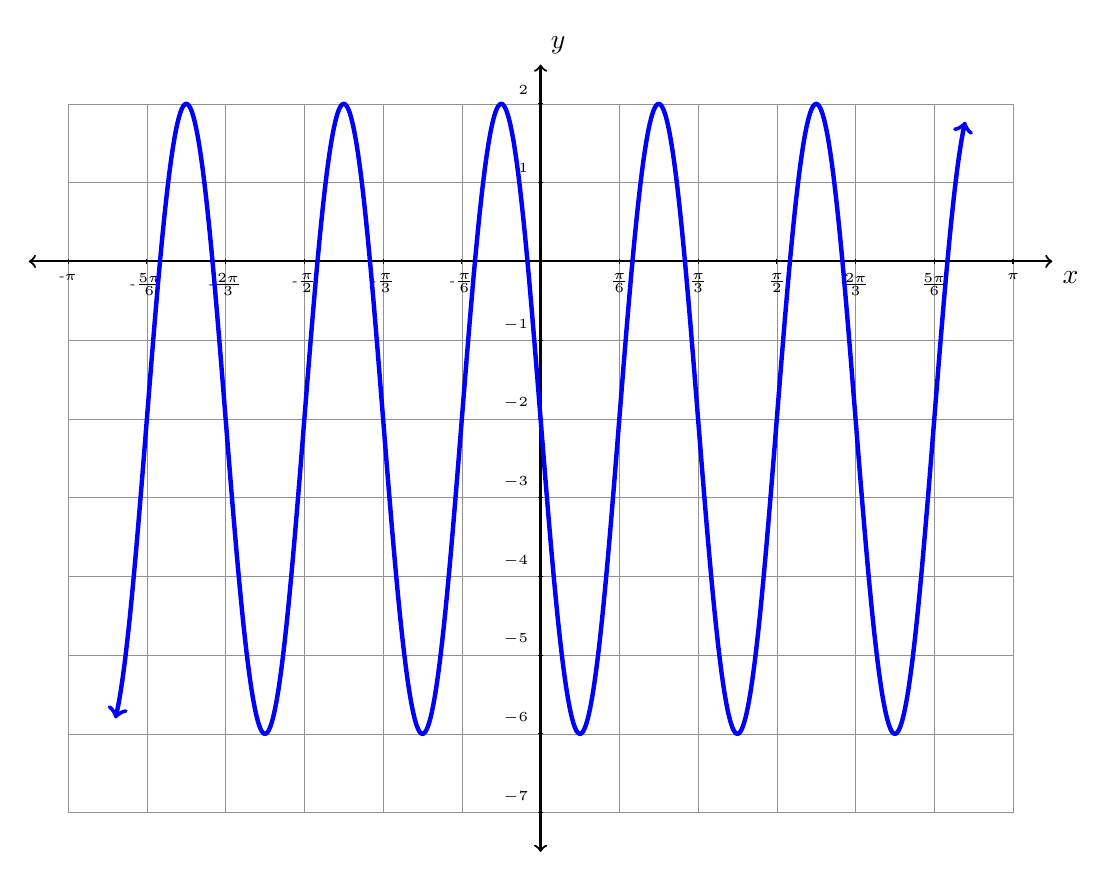
\begin{tikzpicture}[y=1cm, x=1cm,font=\sffamily,
	mydot/.style={
    circle,
    fill=white,
    draw,
    outer sep=0pt,
    inner sep=1.5pt
  }]
    %% Add a grid
    \draw[step = 1, gray, very thin,opacity=0.85] (-6, -7) grid (6, 2);
 	%% Draw the axes
	\draw[thick,<->] (-6.5,0) -- coordinate (x axis mid) (6.5,0) node[anchor = north west] {$x$};
    \draw[thick,<->] (0,-7.5) -- coordinate (y axis mid) (0,2.5) node[anchor = south west] {$y$};
    %% Label the y axis
    \foreach \y in {-7,...,-1,1,2,...,2} {
      \draw (1pt, \y) -- (-1pt, \y) node[anchor = south east] {\tiny $\y$};
    }
    %% Label the x axis
    %\foreach \x in {-5,...,-1,1,2,...,5} {
    %  \draw (\x,1pt) -- (\x,-1pt) node[anchor = north] {\tiny $\x$};
    %}
    \draw (-6,1pt) -- (-6,-1pt) node[anchor = north] {\tiny -$\pi$};
    \draw (-5,1pt) -- (-5,-1pt) node[anchor = north] {\tiny -$\frac{5\pi}{6}$};
    \draw (-4,1pt) -- (-4,-1pt) node[anchor = north] {\tiny -$\frac{2\pi}{3}$};
    \draw (-3,1pt) -- (-3,-1pt) node[anchor = north] {\tiny -$\frac{\pi}{2}$};
    \draw (-2,1pt) -- (-2,-1pt) node[anchor = north] {\tiny -$\frac{\pi}{3}$};
    \draw (-1,1pt) -- (-1,-1pt) node[anchor = north] {\tiny -$\frac{\pi}{6}$};
    \draw (1,1pt) -- (1,-1pt) node[anchor = north] {\tiny $\frac{\pi}{6}$};
    \draw (2,1pt) -- (2,-1pt) node[anchor = north] {\tiny $\frac{\pi}{3}$};
    \draw (3,1pt) -- (3,-1pt) node[anchor = north] {\tiny $\frac{\pi}{2}$};
    \draw (4,1pt) -- (4,-1pt) node[anchor = north] {\tiny $\frac{2\pi}{3}$};
    \draw (5,1pt) -- (5,-1pt) node[anchor = north] {\tiny $\frac{5\pi}{6}$};
    \draw (6,1pt) -- (6,-1pt) node[anchor = north] {\tiny $\pi$};

    %% Draw the function.
    \begin{scope}
%         \draw[very thick,blue] (-3,2) -- (1,1);
%         \draw[very thick,blue] (3.05,1.05) -- (4,3);
%         \draw[very thick,blue] (1.1,4) -- (3,4);
    %semi-circle
         %\draw[very thick, blue] (1,1) arc [radius=1, start angle=180, end angle= 5];
     %parabola
         %\draw[ultra thick, blue, domain=-5:0] plot (\x, {(-0.2)*(\x-5)*(\x+5)});
         \draw[ultra thick, blue, <->, domain=-5.4:5.4] plot[samples=1000] (\x, {-4*sin(pi*\x r)-2});             %dots
%         \fill[blue] (-3, 2) circle[radius=0.5ex];
%         \fill[blue] (1,1) circle[radius=0.5ex];
%         \fill[blue] (4,3) circle[radius=0.5ex];
%         \draw[very thick, blue] (3,1) circle[radius=0.5ex];
%         \fill[blue] (3,4) circle[radius=0.5ex];
%         \draw[very thick, blue] (1,4) circle[radius=0.5ex];


    \end{scope}

    %%\node[above=0.1cm] at (-2,2 )   {\nextXValue};

\end{tikzpicture}


\begin{enumerate}
\item  The graph above is a \textbf{sine} graph that has been transformed.   
\begin{enumerate}

\item  Determine the amplitude, period, phase shift, and vertical shift of function above.

{\bf Amplitude}: \hfill {\bf Period}:\hfill.

\vspace{1cm}

{\bf Phase Shift}: \hfill {\bf Vertical Shift}:\hfill.


\vspace{1cm}
\item  Determine a formula for $f(x)=A\sin(Bx+C)+D$ for the graph above. \vfill
	\vfill
 


\end{enumerate}



\end{enumerate}



